\chapter{Background}
\label{chap:background}

\section{\gls{pow} and \gls{pos}}
In Ethereum, \gls{pos} is aiming to replace \gls{pow} as a distributed consensus
algorithm. This section succintly describes both methods, their main
differences, and which problems arise when you replace \gls{pow} with \gls{pos}.

\subsection{What is \gls{pow}?}
\gls{pow} is the current consensus protocol used to decide between blockchains
in Ethereum. In order to create a new valid block, a node has to solve a
cryptographic puzzle and include its solution in the newly created block. The
difficulty of the puzzle is parametrized in order to output a block on an
average time interval and a reward is given to the creator of each block.  The
consensus rule states that the chain with the greatest total difficulty is to be
considered the main one which incentives miners to build on the main chain if
they want to get rewards for their work. The fact that the difficulty changes to
keep a certain interval between blocks means that work is a proxy for timing; a
miner cannot create an arbitrarily large number of blocks in a short time
because it's inherent to the protocol.


\subsection{What is \gls{pos}?}
\gls{pos} selects a new block creator according to their weight -or stake- which
is determined through the node's age, wealth, etc. In this report, we will
mainly discuss a specific \gls{pos} protocol, \gls{cbc}-Casper.

\subsection{\gls{cbc}-Casper}
\label{ssec:cbc}
\FloatBarrier
\gls{cbc}-Casper \cite{abstractCBC} \cite{abstractCBC2} is an abstract consensus
protocol family which is \gls{pos}-ready. Nodes, called validators in this
context, send messages to each other, acknowledging they saw other messages by
including them in a \textit{justification}, that is attached to each message.
Based on its justification as well as a weighted list of validators, each
message defines an \textit{estimate}, which is the consensus value proposed by
the sender of the message. In the case of a blockchain, each message points to a
single older message as their estimate and form a \textit{block-\gls{dag}}. Running
a slightly modified version of the \gls{ghost} algorithm on the \gls{dag}
\cite{abstractCBC} \cite{GHOST} returns a blockchain.

\begin{figure}[h]
	\centering
	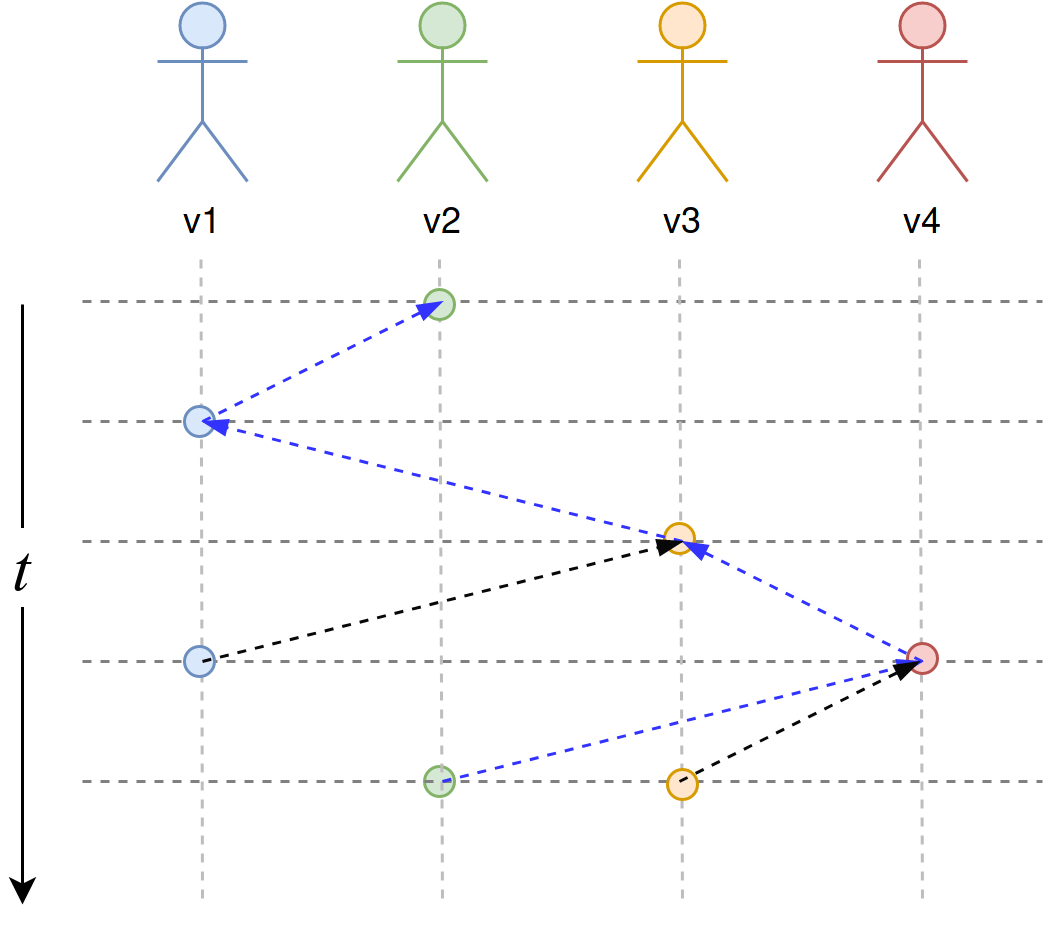
\includegraphics[width=0.8\columnwidth]{cbc-example}
  %\captionsetup{justification=centering}
    \caption{\gls{cbc} blockchain example \todo{comment}}
	\label{fig:example}
\end{figure}

\fig{fig:example} demonstrates a small example of a \gls{cbc} exectution oer a
blockchain with four nodes, messages sent by validators as colored circles,
justifications as dotted arrows, and the selected blockchain with blue arrows.
The blockchain is obtained by running the \gls{ghost} algorithm on the state of
the network as shown in \fig{fig:example} and the result of this algorithm would
be the estimate of a new message sent by an honest validator within this network
state. 

\fig{fig:example2} examplifies validator \(v_1\) producing a new message and the
resulting new blockchain. An honest node includes all the latest messages it has
received (including its own last message).  When a validator does not include
its own messages in its justifications, it is considered as an
\textit{equivocator} which does not follow the protocol, and may be punished by
the network for such a behavior. Note that validator \(v_1\) does not equivocate
because its first message is in the justification of \(v_2\)'s first message,
and \(v_1\) has this message in the justification of its second message. This is
legal because \(v_1\)'s first message is in the dependency of its later
messages.

\textit{Finality} is a key concept to address for this project whereby,
currently a block is considered finalized in a network state if it cannot be
removed by receiving new messages by receiving new messages from honest nodes. 
For \gls{cbc} Casper, a block is considered finalized when a safety oracle is
detected. There are multiple parameters and ways to compute safety oracles and
the one that has been used for this project is: \todo{TODODODODO}

\begin{figure}[h]
	\centering
	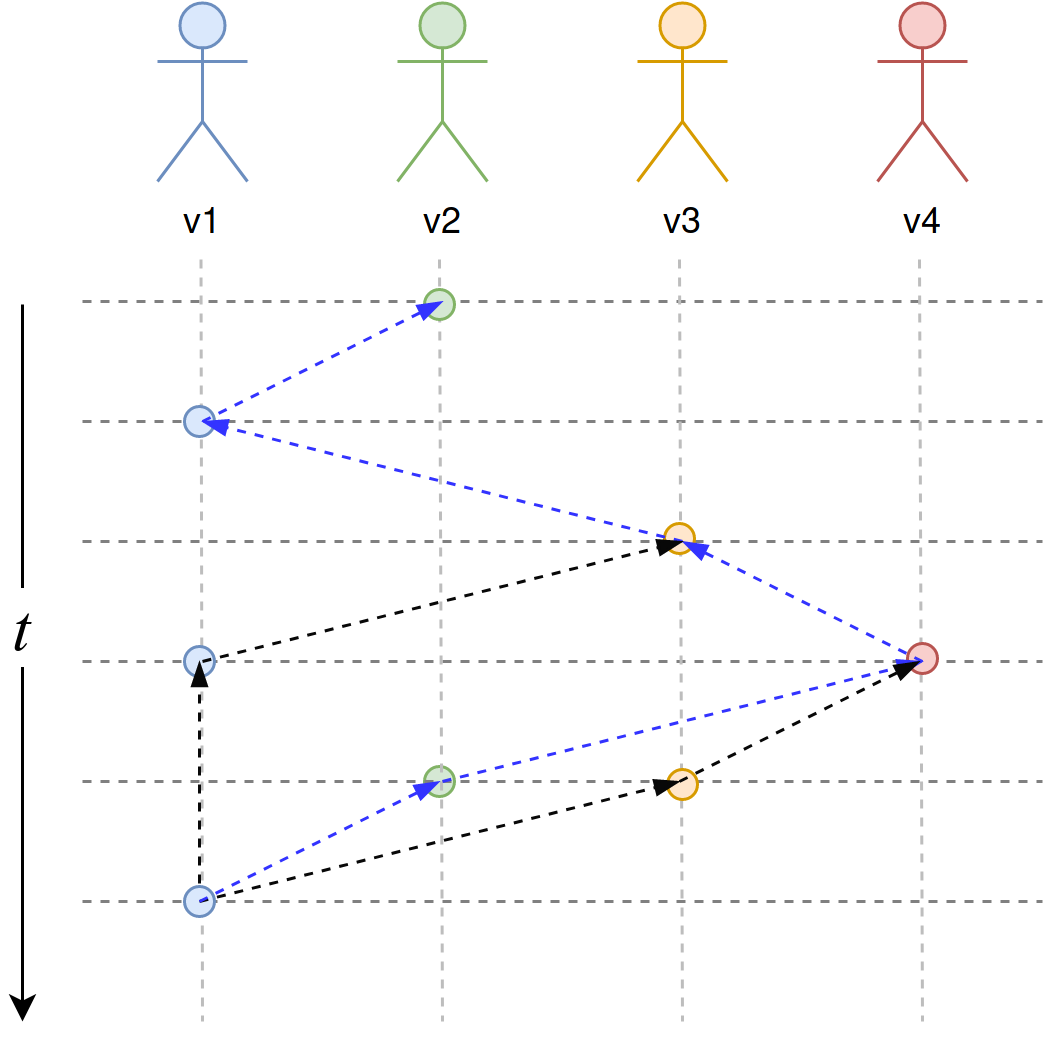
\includegraphics[width=0.8\columnwidth]{cbc-example-2}
  %\captionsetup{justification=centering}
    \caption{\gls{cbc} blockchain example 2 \todo{comment}}
	\label{fig:example2}
\end{figure}

\FloatBarrier
\subsection{Differences between \gls{cbc} Casper and \gls{pow}}
\label{ssec:powVsPos}

\subsubsection{Block production}
In a \gls{pow}\cite{yellowpaper} setting, a miner can broadcast any block to the
network, which will only be picked up by the other nodes if the block is valid,
but the miner has to work to produce said valid block. This restriction implies
that the block miner cannot create blocks at any given time, which is different
to the \gls{cbc} Casper setting that allows nodes to broadcast whenever. 

\subsubsection{Timing assumption}
Time is assumed in a \gls{pow} environment by the amount of work a miner has to
provide to solve a cryptographic puzzle; the difficulty of this puzzle is
determined in such a way that it would require an amount of time to solve that
averages over the network. On the other hand, the \gls{cbc} Casper protocol
family does not make any timing assumption.

\subsubsection{Spam}
The two previous points imply that spamming issues are mitigated by the need to
work to produce blocks in a \gls{pow} chain. However, as there is a negligible
computational cost, a node could easily spam the Casper network.

\subsubsection{Economic majority}
\todo{cite ref, and better explanation}
As machines that are better at solving the cryptographic puzzle in a \gls{pow}
context are more expensive to buy and to operate, \todo{nah}
Economic majority is however built in the \gls{cbc} Casper protocol, in the form
of the weight that validators have.

\subsubsection{Building strategy}
In order to receive a reward for its work, a miner wants a block it has produced
to be included in the main chain. A \gls{pow} protocol usually states that the
chain with the most total difficulty is the main one. Therefore, a miner is
incentivised to build on top of the main chain. 
In a Casper setting, as there is no such incentive, a validator could build on
any chain, or even on its own chain.


\begin{table}[H]
    \centering{
        \begin{tabular}{|l|p{47mm}|p{47mm}|}
            \hline
            & \gls{pow} & \gls{cbc} Casper \\
            \hline
            Block production & Miners can publish blocks if the can prove they
            worked for it & Nodes can publish blocks at any time \\
            \hline
            Timing assumption & Work is a proxy for timing & None \\
            \hline
            Spam & Work removes the possibility to spam & Negligible
            computationnal costs to produce blocks imply potential spam \\
            \hline
            Economic majority & Work is a proxy for economic majority & Economic
            majority \\
            \hline
            Building strategy & Nodes are incentivised to build on the longest
            chain because they have to work to build blocks & No clear
            incentive to build on the longest chain \\
            \hline
        \end{tabular}
        %\captionsetup{justification=centering}
        \caption{Summary of key differences between \gls{pow} and \gls{pos}}
        \label{fig:keyDiffPowPos}
    }
\end{table}

\section{Main problematic}
\todo{rename section}
As seen in \ssec{ssec:powVsPos}, many real-life implementation points are still
to define in order to have a practical \gls{cbc} Casper blockchain. One main
problem that arises is the selection of a block building strategy. This project
will try to propose a model to compare strategies, as well as a framework that
allows one to easily implement new strategies and discuss their performances
based on the proposed model.
Basic strategies that have predictable outputs will be implemented as well, in
order to validate the functionality of the framework.

\section{\texttt{core\_cbc}}
\texttt{core\_cbc} a Rust implementation of the \gls{cbc}-Casper, made by
TrueLevel \todo{introduce somewhere}. It implements the consensus algorithms proposed in the paper and
offers an abstract structure that can be used to create consensus on any value.

\section{Parity Ethereum}
\todo{remove redundancy in this chapter}
\todo{parity networking/gossiping layer research?}
Parity is a Rust Ethereum client. It includes a \textit{Pluggable Consensus}
module that allows one to easily add new consensus protocols by implementing an
interface.  At first, the goal of this project was to implement a small bridge
between the Parity module and the \texttt{core\_cbc} implementation to test block creation
strategies in a pseudo real-like manner. The implementation of the bridge was
not as straight forward as planned so it has been decided to cut it out and test
strategies without mimicking the network and client settings.

\subsection{Background work}
During the early stages of this project, a clear objective was set: to be able
to run a Casper \textit{testnet} with Parity custom nodes. Some work has been
done for the implementation of the \texttt{core-cbc} library into Parity, but
that was left to people that had a better understanding of the underlying
library. Furthermore, considerable effort had been injected in the creation of a
Docker infrastructure in order to easily deploy, connect and monitor multiple
custom Parity nodes on a single machine in order to experiment with different
message building strategies. Using Docker simplified access to the UnNE machine
clusters for testing purposes as software on their clusters are heavily
containerized. After seeing that the Parity implementation would take too much
time to be completed, and therefore might be unusable for this thesis, it has
been decided to evaluate strategies inside the \texttt{core-cbc} library instead
of the more real-life-like setting that is a Parity testnet. The core library
was still being implemented at the time and further testing was needed.  The
main disadvantage of doing the experimentations in the library is that the whole
network latencies and topology are not taken into account. However, a
non-negligible advantage of implementing strategies in the core library is that
it will be easier to test them on consensus values that are not only
blockchains.

\subsection{Local testnet}
Scripts that create and manage two local nodes have been written. They launch 2
Parity instances with the \gls{cbc}-Casper consensus engine, and connect them
to each other. Each node has a user account to send transactions, as well as a
sender account, that can act as a validator in a Casper sense. Currently, each
node produces a block every 10 seconds. This is a basic strategy that enabled
further testing of the Parity inclusion of the \texttt{core-cbc}.

\subsection{Docker testnet}
Testing at a larger scale than two local instances was needed. The possibility
to access a cluster at the UniNE was discussed and the more straightforward way
to run programs on the cluster is to have containers. It was therefore decided
to create a more complex infrastructure using Docker containers.
\texttt{docker-compose} scripts were created to achieve this goal. An arbitrary
number of containers can be created at once and inter-connected in two different
ways:
\begin{itemize}
    \item fully connected;
    \item ring.
\end{itemize}

\begin{figure}
	\centering
	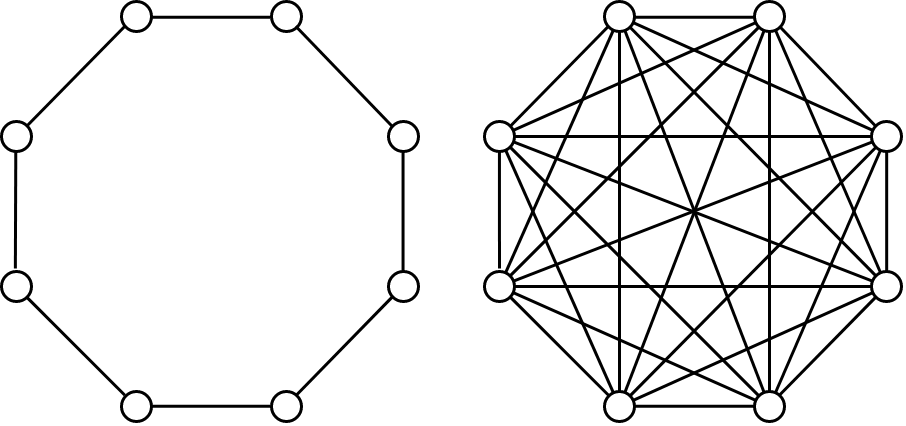
\includegraphics[width=0.8\columnwidth]{rings}
  %\captionsetup{justification=centering}
    \caption{Parity nodes topologies implemented in the Docker testnet. Ring
    layout (left), fully connected (right)}
	\label{fig:layout}
\end{figure}

The created nodes have the same types of accounts as for the local testnet.
In the fully connected setting each node is connected to every other node. In
the ring case, each node is connected to two other nodes in a circular manner.
Those were the two first layouts that were implemented for simplicity. It was
thought to add new layouts afterwards in order to match more precisely the real
network topology of the Ethereum \textit{mainnet}. However, because the Parity
implementation was deemed too time consuming to be used before the end of this
project, no further efforts have been put in that direction. Nevertheless, the
software architecture is in such a state that adding and removing topologies is
easily done through abstract structures.
